\documentclass[10pt]{article}

\usepackage{akteach}
\usepackage{amsmath}
\usepackage{amsfonts}
\usepackage{amssymb}
\usepackage{amsthm}
\usepackage{float}
\usepackage{algpseudocode}
\usepackage[all]{xy}


\newcommand{\C}{\mathbb{C}}
\newcommand{\Q}{\mathbb{Q}}
\newcommand{\K}{\mathbb{K}}
\newcommand{\proj}{\mathbb{P}}
\newcommand{\T}{\mathbb{T}}
\newcommand{\F}{\mathbb{F}}
\newcommand{\Z}{\mathbb{Z}}
\newcommand{\N}{\mathbb{N}}
\newcommand{\cp}{\mathbb{C}P}
\newcommand{\A}{\mathcal{A}}
\newcommand{\BB}{\mathcal{B}}
\newcommand{\CC}{\mathcal{C}}
\newcommand{\NN}{\mathcal{N}}
\newcommand{\MM}{\mathcal{M}}
\newcommand{\E}{\mathcal{E}}
\newcommand{\FF}{\mathcal{F}}
\newcommand{\G}{\mathcal{G}}
\newcommand{\eps}{\varepsilon}
\newcommand{\Hom}{\text{Hom}}
\newcommand{\Div}{\text{div}}
\newcommand{\Res}{\text{Res}}
\newcommand{\ord}{\text{ord}}
\newcommand{\Deg}{\text{deg}}
\newcommand{\mult}{\text{mult}}

\newcommand{\id}{\text{id}}
\newcommand{\Tr}{\text{Tr}}
\newcommand{\ad}{\text{ad}}
\newcommand{\Ad}{\text{Ad}}
\newcommand{\Aut}{\text{Aut}}
\newcommand{\der}{\text{der}}
\newcommand{\GL}{\text{GL}}
\newcommand{\gl}{\mathfrak{gl}}
\newcommand{\rad}{\mathfrak{rad}}
\newcommand{\inhook}{\hookrightarrow}
\newcommand{\sgn}{\text{sign}}

\begin{document}

\akteachheader{Numerical Analysis (CS 450)}%
{Homework Set 3, Bill Karr}

\akteachprobhead{%
  Problem 1: QR iteration with Shifts (11 points)
}

See \verb+cs450hw3p1.py+ for my code. My results were: \begin{verbatim}
Matrix =
[[ 2  3  2]
 [10  3  4]
 [ 3  6  1]]
Computed eigenvalues:  [ 11.  -3.  -2.]
Actual eigenvalues:  [ 11.  -2.  -3.]
Matrix =
[[6 2 1]
 [2 3 1]
 [1 1 1]]
Computed eigenvalues:  [ 7.28799214  2.13307448  0.57893339]
Actual eigenvalues:  [ 7.28799214  2.13307448  0.57893339]
\end{verbatim}

\akteachprobhead{%
  Problem 2: Lanczos Iteration and Convergence of Ritz Values (31 points)
}

\begin{enumerate}

\item[(a)] Prove that, in the case of $A$ symmetric and real-valued, Arnoldi iteration reduces to Lanczos iteration.

\begin{proof}
We know that both iterations output matrices $H$ and $Q$, given $A$, where $ H $ is in upper Hessenberg form, $Q$ is an orthogonal matrix, and $ H = Q^T A Q $.

However, notice that $ H^T = ( Q^T A Q )^T = Q^T A^T (Q^T)^T = Q^T A Q = H$. Thus, $H$ is symmetric.

In addition, since $H$ is upper Hessenberg and symmetric, the entries above the first super-diagonal are zeros since the entries below the first sub-diagonal are zeros. 

Finally, since the entries above the first super-diagonal are zero, then the $j$ loop in Arnoldi iteration, as show in Algorithm 4.9 in the book, is trivial except when $ j = k-1 $ and $ j = k $ since $ h_{jk} = 0 $ whenever $ | j - k | > 1 $. Hence, only two iterations are needed in the $j$ loop. 

This is exactly what the Lanczos algorithm produces, so Arnoldi reduces to Lanczos when $A$ is symmetric.
\end{proof}

\item[(b)] See \verb+cs450hw3p2.py+ for my code. My results were: \begin{verbatim} 
size(A) = 25 by 25
|QQ.T - I| = 7.21487455622e-07
|Q.T*A*Q - H|/|A| = 3.02974383378e-07 
\end{verbatim}

It's worth noting that these errors are not very small even though $A$ is only a 25 by 25 matrix, demonstrating the numerical instability of Lanczos iteration.

\item[(c)] See \verb+cs450hw3p2.py+ for my code. See the figure below for the plots of the Ritz values.

\begin{figure}[H]
  \centering
    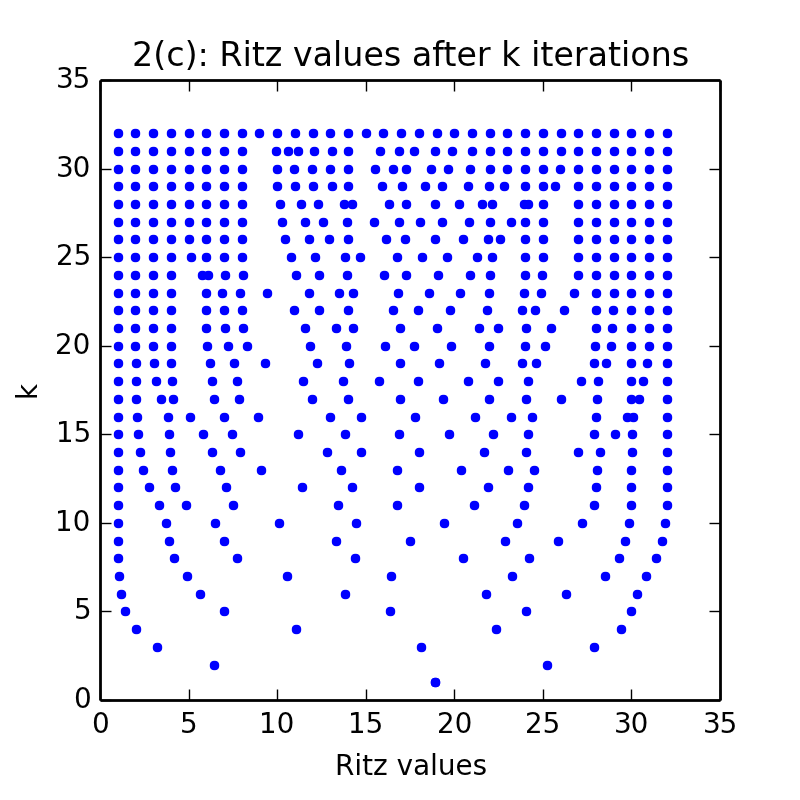
\includegraphics[scale=0.8]{p2fig1}
\end{figure}

\end{enumerate}

\akteachprobhead{%
  Problem 3: Reduction to Hessenberg form (25 points)
}

\begin{enumerate}

\item[(a)] Let $ A \in \R^{n \times n} $ be a matrix. Also, let $H$ be a Householder reflector designed to annihilate rows $ 3, ... , n $ of the first column of $A$. 

Show that the matrix $ B = HAH^T $ has the form \begin{equation}
B = \begin{pmatrix}
* & * & \cdots & * \\
* & * & \cdots & * \\
0 & * & \cdots & * \\
\vdots & \vdots & \ddots & \vdots \\
0 & * & \cdots & *
\end{pmatrix}
\end{equation} i.e. it has zeros below the second diagonal of the first column. You may assume that $HA$ has the non-zero pattern in (1).

\begin{proof}
The vector $v$ used to compute the Householder transformation is of the form $$
v = \begin{pmatrix}
0 \\
0 \\
* \\
\vdots \\
*
\end{pmatrix}.
$$ Thus, $H = I - 2 \frac{v v^T}{v^T v}$ is of the form $$
H = \begin{pmatrix}
1 & 0 & \cdots & 0 & 0 \\
0 & 1 & \cdots & 0 & 0 \\
\vdots & \vdots & \ddots & \vdots & 0 \\
0 & 0 & \cdots & 1 & 0 \\
0 & 0 & \cdots & 0 & 1
\end{pmatrix} - 
\begin{pmatrix}
0 & 0 & 0 & \cdots & 0 \\
0 & 0 & 0 & \cdots & 0 \\
0 & 0 & * & \cdots & * \\
\vdots & \vdots & \vdots & \ddots & \vdots \\
0 & 0 & * & \cdots & *
\end{pmatrix} =
\begin{pmatrix}
1 & 0 & 0 & \cdots & 0 \\
0 & 1 & 0 & \cdots & 0 \\
0 & 0 & * & \cdots & * \\
\vdots & \vdots & \vdots & \ddots & \vdots \\
0 & 0 & * & \cdots & *
\end{pmatrix}
$$ Furthermore, since $H^T = H$ and $HA$ is of the form in (1), we use matrix multiplication and find that $ HAH^T $ is of the form $$
HAH^T = (HA)H = \begin{pmatrix}
* & * & * & \cdots & * \\
* & * & * & \cdots & * \\
0 & * & * & \cdots & * \\
\vdots & \vdots & \vdots & \ddots & \vdots \\
0 & * & * & \cdots & *
\end{pmatrix}
\begin{pmatrix}
1 & 0 & 0 & \cdots & 0 \\
0 & 1 & 0 & \cdots & 0 \\
0 & 0 & * & \cdots & * \\
\vdots & \vdots & \vdots & \ddots & \vdots \\
0 & 0 & * & \cdots & *
\end{pmatrix} = \begin{pmatrix}
* & * & * & \cdots & * \\
* & * & * & \cdots & * \\
0 & * & * & \cdots & * \\
\vdots & \vdots & \vdots & \ddots & \vdots \\
0 & * & * & \cdots & *
\end{pmatrix}
$$ This completes the proof.
\end{proof}

\item[(b)] See \verb+cs450hw3p3.py+ for my code.

\item[(c)] See \verb+cs450hw3p3.py+ for my code. My results were \begin{verbatim}
|Q.T*U*Q - A|/|A| = 6.53919429383e-16
\end{verbatim}

\item[(d)] See \verb+cs450hw3p3.py+ for my code. My results were \begin{verbatim}
|Q.T*U*Q - A|/|A| = 8.03225086772e-16
|QQ.T - I| = 1.5667118603e-15 <-- when this is small, Q is orthogonal
|U.T - U|/|U| = 7.97339107923e-17 <-- when this is small, U is symmetric
\end{verbatim}

Thus, $ U $ is upper Hessenberg, but it is also symmetric and therefore also in ``lower Hessenberg" form. It's a tridiagonal symmetric matrix.

\end{enumerate}

\akteachprobhead{%
  Problem 4: Newton's method in 1D (18 points)
}

\begin{enumerate}

\item[(a)] Newton's method for solve a scalar nonlinear equation $f(x) = 0$ requires computation of the derivative of $f$ at each iteration. Suppose that we instead replace the true derivative with a constant value $ d $, that is, we use the iteration scheme: $$
x_{k+1} = x_k - f(x_k)/d.
$$ 

\begin{enumerate}
\item[(i)] Under what conditions on the value of $d$ will this scheme be locally convergent.

\begin{proof}[Solution]
By Taylor's theorem, we can approximate $f$ near the root $x^*$ so that for small $ \eps $, we have $$
f(x^* + \eps) = f'(x^*) \eps + O(\eps^2).
$$ Thus, $$
x_{k+1} - x^* = x_k - x^* - \frac{f'(x^*) (x_k - x^*) + O((x_k - x^*)^2)}{d} $$ $$\Rightarrow e_{k+1} = e_{k} \left( 1 - \frac{f'(x^*)}{d} \right) + O(e_{k}^2) \Rightarrow \left| \frac{e_{k+1}}{e_k} \right| = \left|  1 - \frac{f'(x^*)}{d} + O( e_k ) \right| $$ In order to converge locally we must have, $ \left| 1 - \frac{f'(x^*)}{d} \right| < 1 $ so $ 0 < \frac{f'(x^*)}{d} < 2 $ or equvalently $ \frac{d}{f'(x^*)} > \frac{1}{2} $. Thus, $d$ must have the same sign as the derivative at the root $ f'(x^*) $ and it cannot be too small relative to the derivative.
\end{proof}

\item[(ii)] What will be the convergence rate in general?

\begin{proof}[Solution]
By the above, we have $$
\frac{|e_{k+1}|}{|e_k|} \approx \left| 1 - \frac{f'(x^*)}{d} \right| + O(|e_k|),
$$ so in general, this method should have a linear convergence rate.
\end{proof}

\item[(iii)] Is there any value of $d$ that would still yield quadratic convergence?

\begin{proof}[Solution]
Notice that if the linear convergence rate $ \left| 1 - \frac{f'(x^*)}{d} \right| $ is zero, then we actually have quadratic convergence. This happens exactly when $ d = f'(x^*) \neq 0 $. So, we $d$ is the derivative of $f$ at the root and the root is order 1, then this method yields quadratic convergence, locally.
\end{proof}

\end{enumerate}

\item[(b)] See \verb+cs450hw3p4.py+ for my code. My code prints out a list of $r $ values, one computed at each iteration. The last few $r$ values printed should show the true $r$ value. I used the following formula for $r$ at each iteration: $$
r = \frac{\log(e_{k+1}/e_k)}{\log(e_k/ e_{k-1})}
$$ where $ e_k = | x_k - x^* | $.

\begin{enumerate}
\item[(i)] For $ f(x) = x^2 - 1 $, the observed convergence rate is quadratic, i.e. $r = 2$. The reason is because the root it's converging to is $ x^* = 1 $ which has multiplicity 1. Thus, Newton's method has quadratic convergence.

\item[(ii)] For $ f(x) = (x-1)^4 $, the observed convergence rate is linear, i.e. $r = 1$. This is because it is converging to $ x* = 1 $ which has multiplicity $ 4 $ which is larger than 1. Thus, Newton's method has linear convergence in this case.

\item[(iii)] For $ f(x) = x - \cos(x) $, the observed convergence rate is quadratic, i.e. $r = 2$. The reason is because the root it's converging to has multiplicity 1 since $ f'(x*) = 1 - \sin(x^*) = 1 \mp \sqrt{1 - (x^*)^2} \neq 0 $. You can easily see this if you plot the graph of $ f(x) = x - \cos(x) $. Thus, Newton's method has quadratic convergence.

\begin{figure}[H]
  \centering
    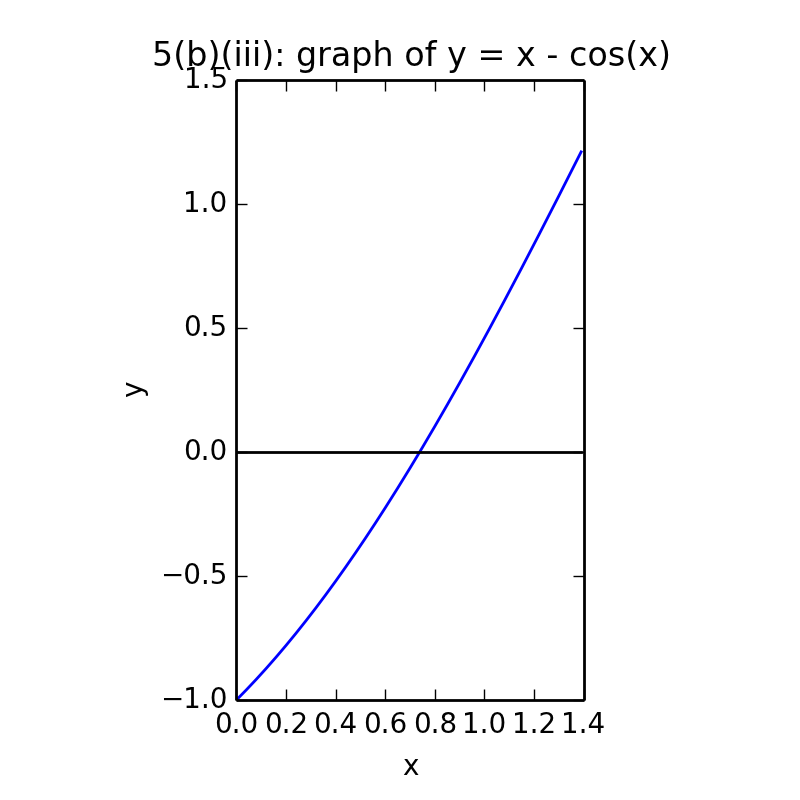
\includegraphics[scale=0.8]{p5fig1}
\end{figure}

\end{enumerate}

\end{enumerate}

\akteachprobhead{%
  Problem 5: Newton's method for a system (15 points)
}

\begin{enumerate}

\item[(a)] See \verb+cs450hw3p5.py+ for my code.

\item[(b)] See \verb+cs450hw3p5.py+ for my code.

\item[(c)] See \verb+cs450hw3p5.py+ for my code. 

The relative error is not necessarily small when the relative residual is small. This is because, given a vector in Cartesian coordinates, there are multiple ways to represent the point in spherical coordinates and Newton's method doesn't always converge to the ``standard" spherical coordinates; it is only guaranteed to converge to a set of numbers $ (r, \theta, \varphi) $ that satisfy $ f(r, \theta, \varphi) = 0 $ which has infinitely many solutions. For example, if you shift $\theta$ by a multiple of $2 \pi$ or if you shift $ \varphi $ by a multiple of $\pi$, you will not change the Cartesian point represented. 

Here are my results as printed from my code:

\begin{verbatim}
Trial 1

Number of iterations of Newton's method: 7
Cartesian vector = [ 0.47298583 -0.68142588  0.2424395 ]

Output using Newton's method = [-0.86419543  1.85515071  2.17755962]
 True spherical coordinates  = [ 0.86419543  2.47917726 -0.96403303]

relative residual = 2.89055198425e-16
relative error = 1.30129251914

Trial 2

Number of iterations of Newton's method: 10
Cartesian vector = [-1.70073563  0.75314283 -1.53472134]

Output using Newton's method = [ -2.41145089   0.88093441 -31.8328049 ]
 True spherical coordinates  = [ 2.41145089  1.25316277  2.72471429]

relative residual = 6.70347104211e-16
relative error = 9.06744023065

Trial 3

Number of iterations of Newton's method: 6
Cartesian vector = [ 0.00512708 -0.12022767 -0.80698188]

Output using Newton's method = [ 0.81590485 -2.99356369  1.61341525]
 True spherical coordinates  = [ 0.81590485  1.71868988 -1.52817741]

relative residual = 4.17291477464e-16
relative error = 2.32083829101

Trial 4

Number of iterations of Newton's method: 9
Cartesian vector = [ 2.87181939 -0.59782292  0.47245699]

Output using Newton's method = [ 2.97118739  1.41110562 -6.48842291]
 True spherical coordinates  = [ 2.97118739  1.77338602 -0.2052376 ]

relative residual = 2.17881143295e-16
relative error = 1.81567932411

Trial 5

Number of iterations of Newton's method: 10
Cartesian vector = [ 1.09595612 -1.2151688   1.34235637]

Output using Newton's method = [ 2.11652443  0.88378837 -0.83693459]
 True spherical coordinates  = [ 2.11652443  2.18234248 -0.83693459]

relative residual = 1.48365162969e-16
relative error = 0.411819309513

Trial 6

Number of iterations of Newton's method: 6
Cartesian vector = [-0.12214979  1.01251548 -0.91386915]

Output using Newton's method = [ 1.36940315  2.30143914  1.69085604]
 True spherical coordinates  = [ 1.36940315  0.73864059  1.69085604]

relative residual = 1.67137296585e-16
relative error = 0.680130495471

Trial 7

Number of iterations of Newton's method: 6
Cartesian vector = [-1.02953021  1.20979645  0.5018723 ]

Output using Newton's method = [ 1.66595789  1.26479148  2.27586751]
 True spherical coordinates  = [ 1.66595789  0.7580374   2.27586751]

relative residual = 1.88491253438e-16
relative error = 0.173513265511

Trial 8

Number of iterations of Newton's method: 5
Cartesian vector = [ 0.13884618  0.64076111  0.52733267]

Output using Newton's method = [ 0.84138743  0.89343152  1.35740592]
 True spherical coordinates  = [ 0.84138743  0.70509036  1.35740592]

relative residual = 6.26794132391e-13
relative error = 0.107885648614

Trial 9

Number of iterations of Newton's method: 28
Cartesian vector = [-1.15436024 -2.21333348 -1.68175651]

Output using Newton's method = [ -3.00993316  55.57073176 -14.61790418]
 True spherical coordinates  = [ 3.00993316  2.3969691  -2.05153357]

relative residual = 1.13328561435e-15
relative error = 12.6061490462

Trial 10

Number of iterations of Newton's method: 20
Cartesian vector = [-1.78809425 -2.21853495 -0.64743078]

Output using Newton's method = [ 2.92204466  4.48896712  0.89241981]
 True spherical coordinates  = [ 2.92204466  2.4329418  -2.24917284]

relative residual = 4.5524744551e-14
relative error = 0.849888371936
\end{verbatim}

\end{enumerate}

\end{document}
